\section{Infinite Groups and Representations}

The way of writing down representations of groups that was introduced in the last section does not work for all groups and representations.
If the group has an infinite number of conjugacy classes, we cannot write down the character.
Also if the representation is infinite-dimensional, meaning the vector space its elements act on is infinite-dimensional, the trace may not be defined.
So we can't write down the character either.
In this section we encounter examples for both cases, starting with an infinite group.

\subsection{Infinite Group}

First, we want to define a representation of an infinite group.
$S^1$ is an easy-to-understand group with a simple structure.
It consists of all rotational symmetries of a circle, like the unit circle in \Cref{fig:infinite.group.unit}.
One \textit{simple} (irreducible) and \textit{faithful} representation is the identification of each rotation with its angle $\theta$.
The (counterclockwise) rotation is represented by the number $e^{\theta i}$.
This representation is one-dimensional and faithful.
We can see that $S^1$ must be abelian since the complex numbers commute under multiplication.
One result of Shur's Lemma introduced in \Cref{sec:reprep.simp} is that all simple representations of abelian groups must be one-dimensional~\cite{hein2013}.


\begin{figure}[!h]
    \centering

    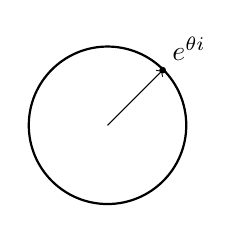
\begin{tikzpicture}
        \draw[thick] (0,0) circle (1);

        \coordinate (z) at (0.7, 0.7);
        \draw[fill] (z) circle (1pt);
        \draw[->] (0,0) -- (z);

        \node[above right] at (z) {$e^{\theta i}$};
    \end{tikzpicture}

    \caption{Unit Circle with a Complex Number}
    \label{fig:infinite.group.unit}
\end{figure}

\subsection{Infinite Representation}

An example of an infinite-dimensional representation of a group would be the infinite-dimensional representation of the group $\text{SL}_2(\mathbb{R})$.
It is the group of all $2 \times 2$ real matrices with a determinant of one.
From this definition, you can immediately see, that there exists at least one finite-dimensional representation of this group.

To describe this infinite-dimensional representation, we first need to find generators of the group $\text{SL}_2(\mathbb{R})$.
In this case, there are three and we will call them $E$, $F$, and $H$.
They need to satisfy the following equations:
\begin{subequations}
    \begin{align}
        [H, E] & = 2E \\
        [H, F] & = -2F \\
        [E, F] & = H
    \end{align}
\end{subequations}
where $[A, B] = A \cdot B - B \cdot A$ is the so called commutator of $A$ and $B$.
The matrices satisfying these equations are
\begin{align}
    H = -i \cdot \begin{pmatrix}
        0 & 1 \\
        -1 & 0
    \end{pmatrix}, \qquad
    E = \frac{1}{2} \cdot \begin{pmatrix}
        1 & i \\
        -i & 1
    \end{pmatrix}, \text{ and} \qquad
    F = \frac{1}{2} \cdot \begin{pmatrix}
        1 & -i \\
        -i & 1
    \end{pmatrix} 
\end{align}

For the representation, we need an infinite-dimensional vector space $V$.
We don't need to think about what it looks like, just assume it has an infinite number of basis vectors $\{\ldots, v_{-1}, v_0, v_1, \ldots\}$.
We now construct a representation on a subspace of this vector space $V$ by choosing a $\lambda \in \C$.
The representation $\rho(a) \in \GL(V)$ of an action $a \in \text{SL}_2(\mathbb{R})$ is then given by
\begin{subequations}
    \begin{align}
        \rho(H) \cdot v_n & = n \cdot v_n \\
        \rho(E) \cdot v_n & = \frac{\lambda + n + 1}{2} \cdot v_{n + 2} \\
        \rho(F) \cdot v_n & = \frac{\lambda - n - 1}{2} \cdot v_{n - 2}
    \end{align}
\end{subequations}
where $n \in \mathbb{Z}$.
To obtain the representation $\rho(a)$ for any action $a \in \text{SL}_2(\mathbb{R})$, you first need to write it as some combination of $H$, $E$, and $F$ then you can combine the given linear for every element given above like you combined the elements.
From these three formulas, one can see that the resulting maps on $V$ are indeed linear.
Also, we don't need all basis vectors, we only need either all the ones with even indices or the ones with odd indices~\cite{borcherds2011}.

These representations are irreducible, if and only if neither $\rho(E) \cdot v_n = 0$ nor $\rho(F) \cdot v_n = 0$ for some $n$.
Otherwise, there would be an opportunity to cut the vector space around that index $n$.
Such a thing happens if $\lambda \in \mathbb{Z}$.
So if we choose $\lambda \in \C \setminus \mathbb{Z}$, the representation above will be infinite and irreducible~\cite{borcherds2011}.

